\section{Результаты измерений}

\begin{figure}[ht!]
    \centering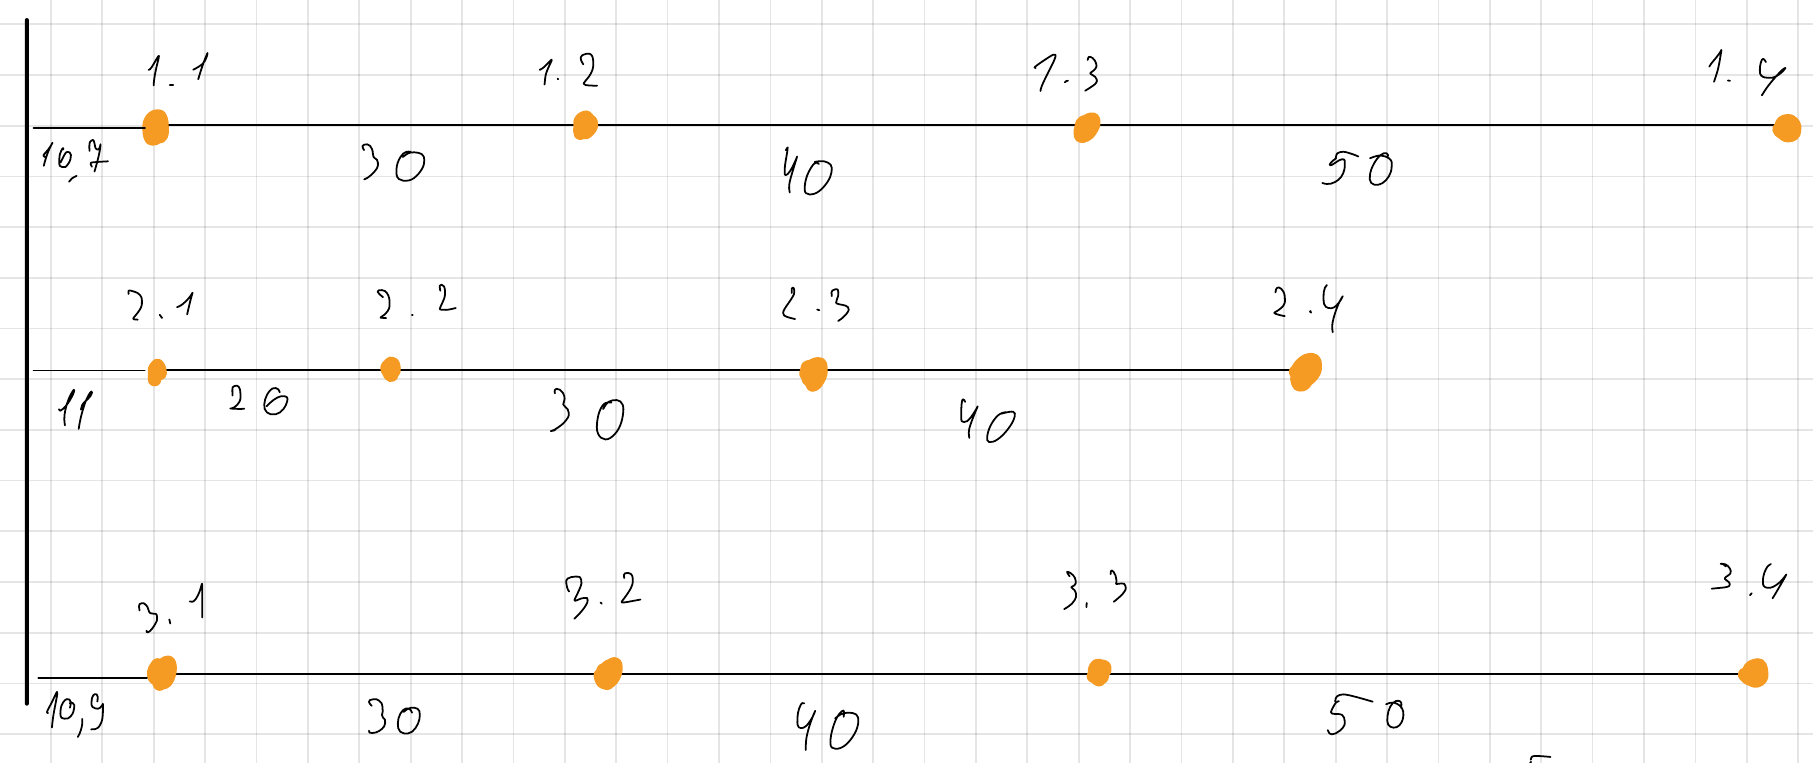
\includegraphics[width=0.8\linewidth]{img/eq2.png}
\end{figure}

Расстояния между местами подсоединения микроманометра указаны на рисунке.

Диаметры трубок:
\begin{enumerate}
    \item $d_1=5{,}1\pm 0{,}05\,\text{мм}$
    \item $d_2=3{,}0\pm 0{,}1\,\text{мм}$
    \item $d_3=3{,}95\pm 0{,}05\,\text{мм}$
\end{enumerate}

Параметры окружающей среды:
\begin{gather}
    t=23{,}1\,^\circ \mathrm{C} \\
    \varphi = 30{,}4\,\% \\
    p_\text{атм} = 98{,}54\,\text{КПа}
\end{gather}

Определим случайную погрешность измерения времени. Для этого установим некоторый расход
воздуха и будем измерять время, за которое счетчик изменит показания на $5\,\text{л}$:
\begin{table}[ht!]
    \centering
\begin{tabular}{|l|l|l|l|l|l|l|l|}
    \hline
    $t,\text{с}$ & 43.82 & 43.77 & 43.9 & 43.92 & 43.82 & 43.94 & 43.86 \\ \hline
    \end{tabular}
\end{table}

\[\Delta t\approx 0{,}02\,\text{с}\]
\[\varepsilon_t\approx 3\cdot 10^{-4}\]

Погрешность измерения объема составляет $0{,}01$, поэтому при измерении расхода на 5 л можно
пренебречь погрешностью измернеия времени.

\[Q_\text{кр}\approx 5\cdot 10^{-2}\,\text{л}/\text{с}\]
\[\Delta p_\text{кр}\approx 800\,\text{Па}\]
\[l_\text{уст}\approx 20\,\text{см}\]

\begin{table}[!ht]
    \centering
    \begin{tabular}{|l|l|l||l|l|l||l|l|l|}
    \hline
        $Q_1,\,\text{л}/\text{с}$ & $h_1\,\pm 0{,}5$ & $a_1$ & $Q_2,\,\text{л}/\text{с}$ & $h_2\,\pm 0{,}5$ & $a_2$ & $Q_3,\,\text{л}/\text{с}$ & $h_3\,\pm 0{,}5$ & $a_3$ \\ \hline
        0.2064 & 80 & 0.2 & 0.0279 & 25 & 0.3 & 0.0194 & 15 & 0.2 \\ \hline
        0.19175 & 70 & 0.2 & 0.04778 & 50 & 0.3 & 0.03877 & 31 & 0.2 \\ \hline
        0.17727 & 60 & 0.2 & 0.6552 & 75 & 0.3 & 0.054466 & 44 & 0.2 \\ \hline
        0.162 & 50 & 0.2 & 0.809 & 100 & 0.3 & 0.073877 & 60 & 0.2 \\ \hline
        0.145 & 40 & 0.2 & 0.055 & 60 & 0.3 & 0.0833 & 75 & 0.2 \\ \hline
        0.12934 & 29 & 0.2 & 0.0407 & 40 & 0.3 & 0.1 & 90 & 0.2 \\ \hline
        0.2225 & 91 & 0.2 & 0.06785 & 80 & 0.3 & 0.06134 & 50 & 0.2 \\ \hline
        & & & & & & 0.04862 & 40 & 0.2 \\ \hline
    \end{tabular}
\end{table}

\[\Delta p = K \cdot h \cdot a\]
$K=9.80665\,\text{Па}$, $\varepsilon_a \approx 1\,\%$

\begin{figure}[ht!]
    \centering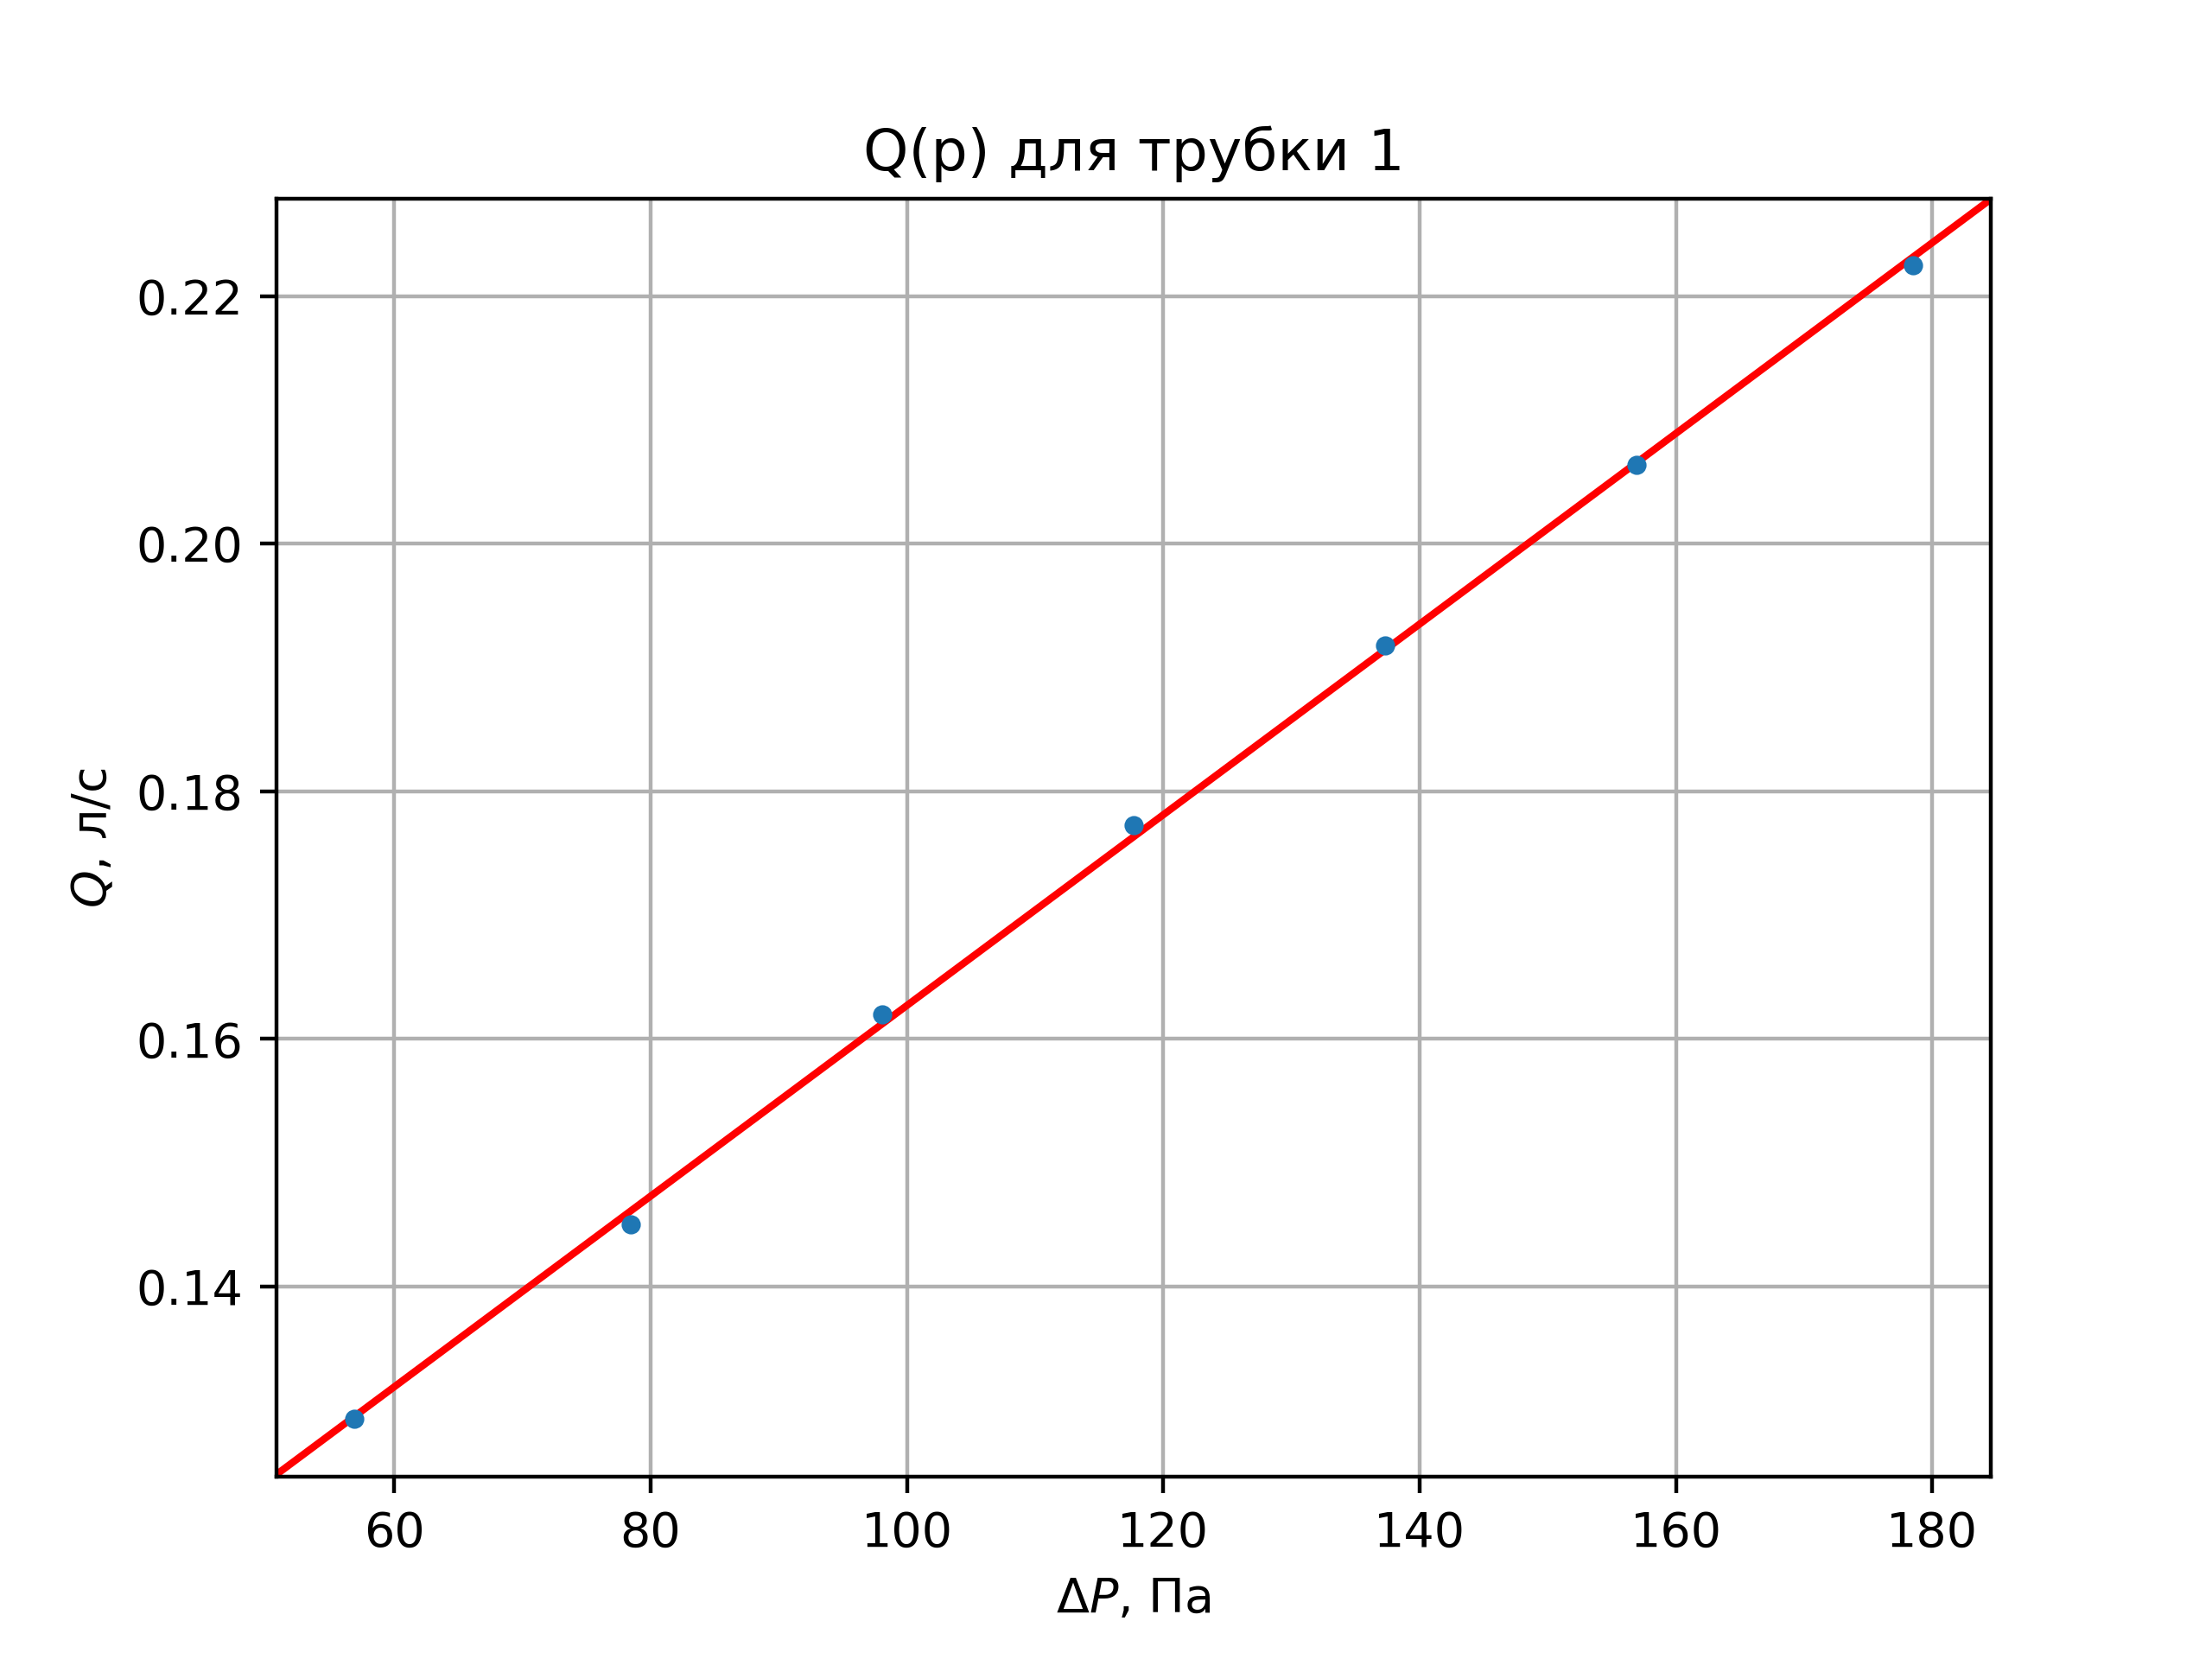
\includegraphics[width=0.6\linewidth]{img/data01.png}
    \centering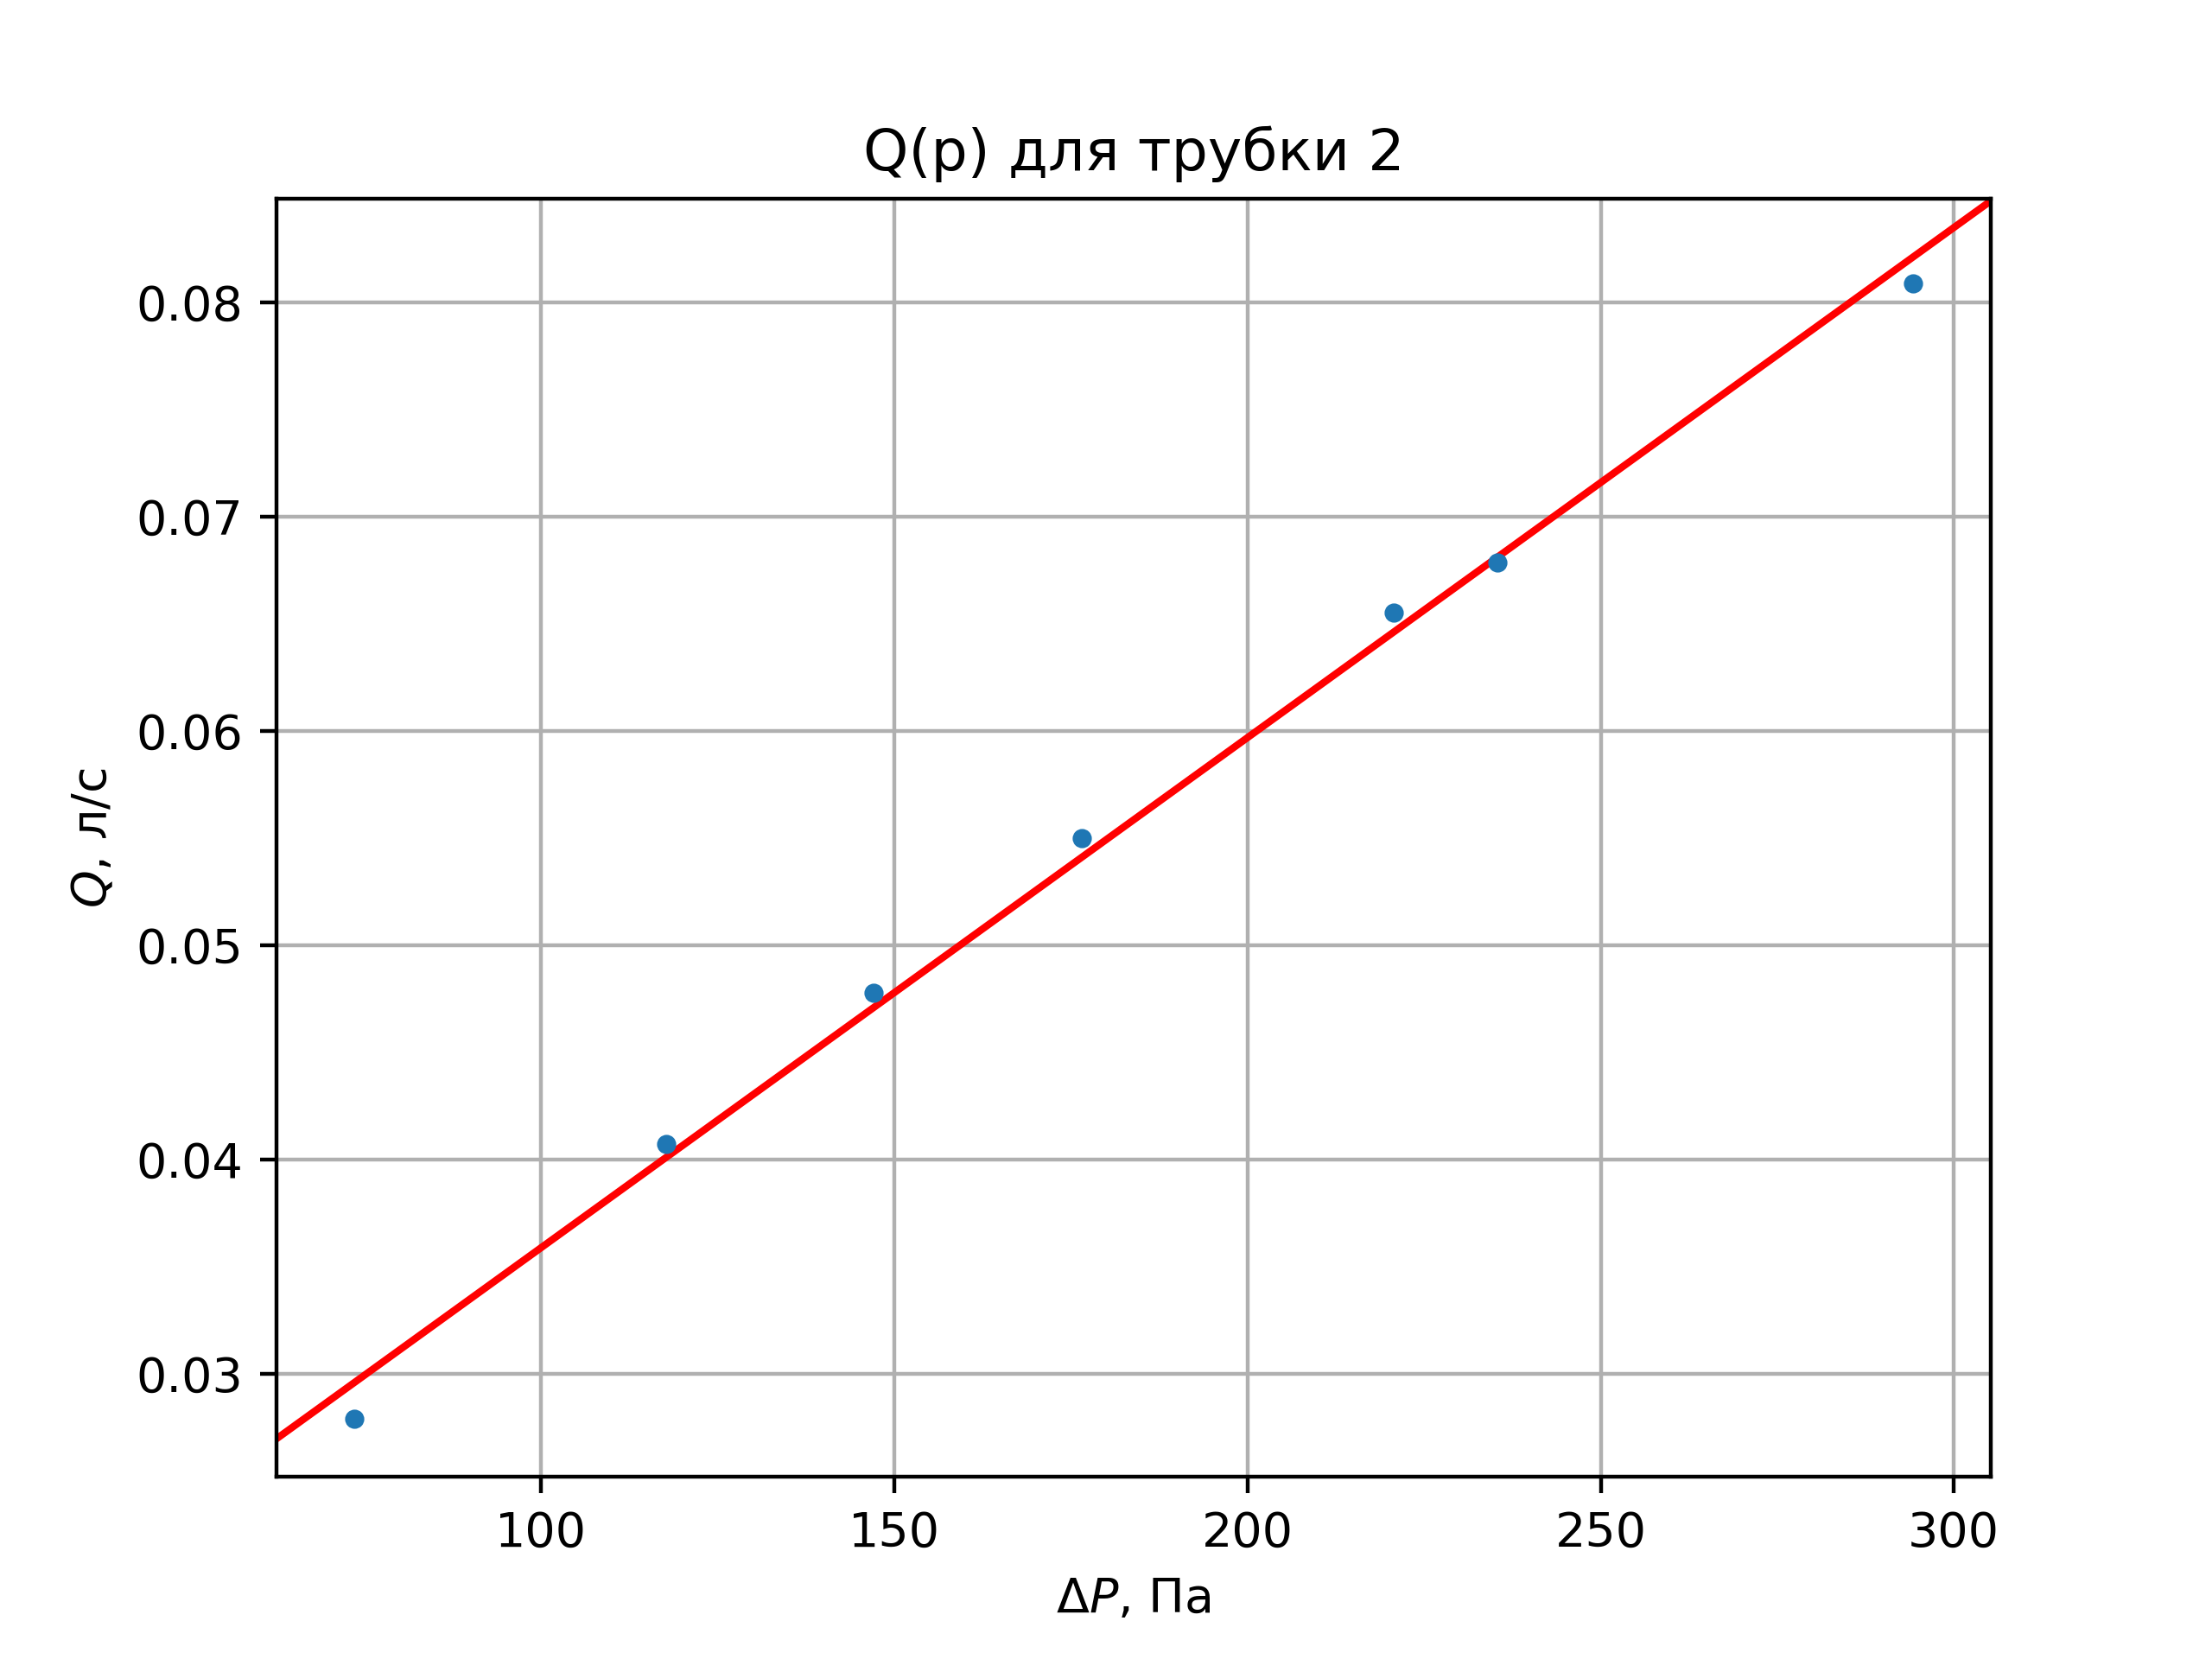
\includegraphics[width=0.6\linewidth]{img/data02.png}
    \centering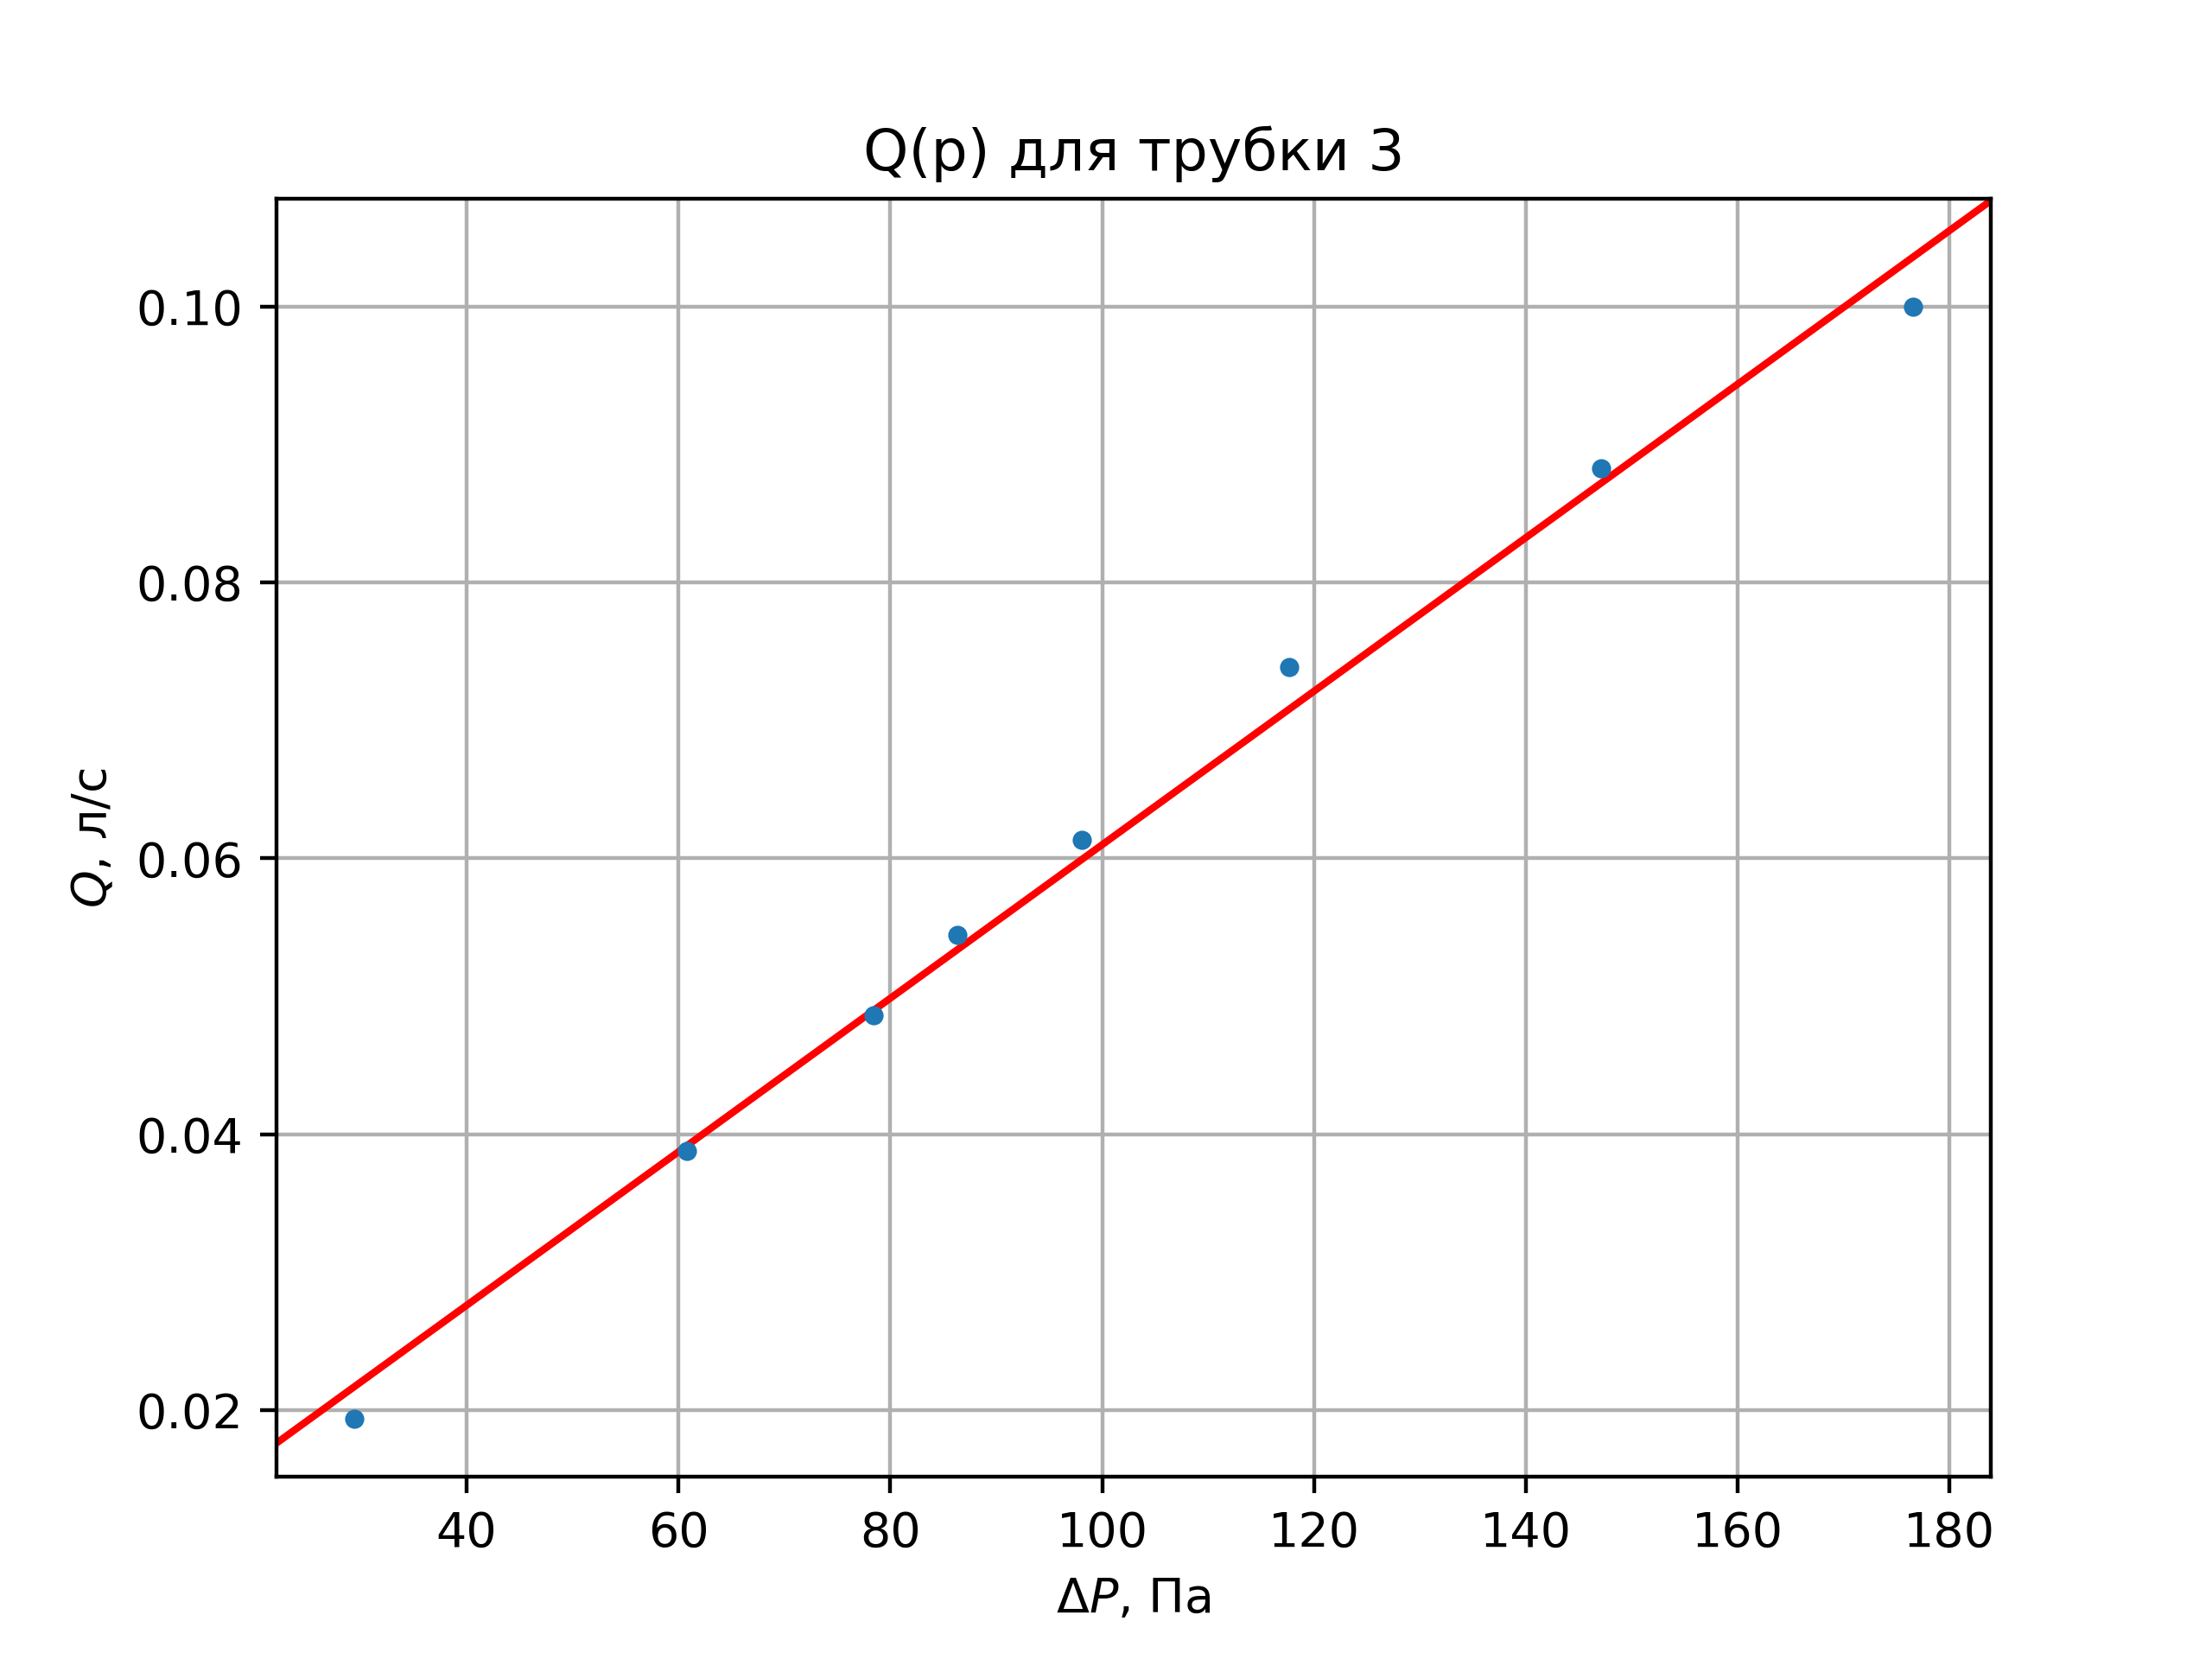
\includegraphics[width=0.6\linewidth]{img/data03.png}
\end{figure}

Из графиков
\[\eta_1 = \left(5{,}4\pm 0{,}4\right)\cdot 10^{-5}\,\text{Па}\cdot\text{с}\]
\[\eta_2 = \left(2{,}8\pm 0{,}5\right)\cdot 10^{-5}\,\text{Па}\cdot\text{с}\]
\[\eta_3 = \left(2{,}1\pm 0{,}2\right)\cdot 10^{-5}\,\text{Па}\cdot\text{с}\]

Табличное значение вязкости $1{,}8\cdot 10^{-5}\,\text{Па}\cdot\text{с}$

\begin{table}[!ht]
    \centering
    \begin{tabular}{|l|l|l||l|l|l||l|l|l|}
    \hline
        $l_1,\,\text{см}$ & $h_1\pm 0{,}5$ & $a_1$ & $l_2,\,\text{см}$ & $h_2\pm 0{,}5$ & $a_2$ & $l_3,\,\text{см}$ & $h_3\pm 0{,}5$ & $a_3$ \\ \hline
        50 & 116 & 0.2 & 30 & 100 & 0.3 &  50 & 80 & 0.2\\ \hline
        40 & 91 & 0.2 & 20 & 76 & 0.3 & 40 & 87 & 0.2 \\ \hline
        30 & 85 & 0.2 & 11 & 112 & 0.3 & 30 & 60 & 0.2\\ \hline
        10.7 & 102 & 0.2 & & & & 10.9 & 54 & 0.2 \\ \hline
    \end{tabular}
\end{table}

\begin{figure}[ht!]
    \centering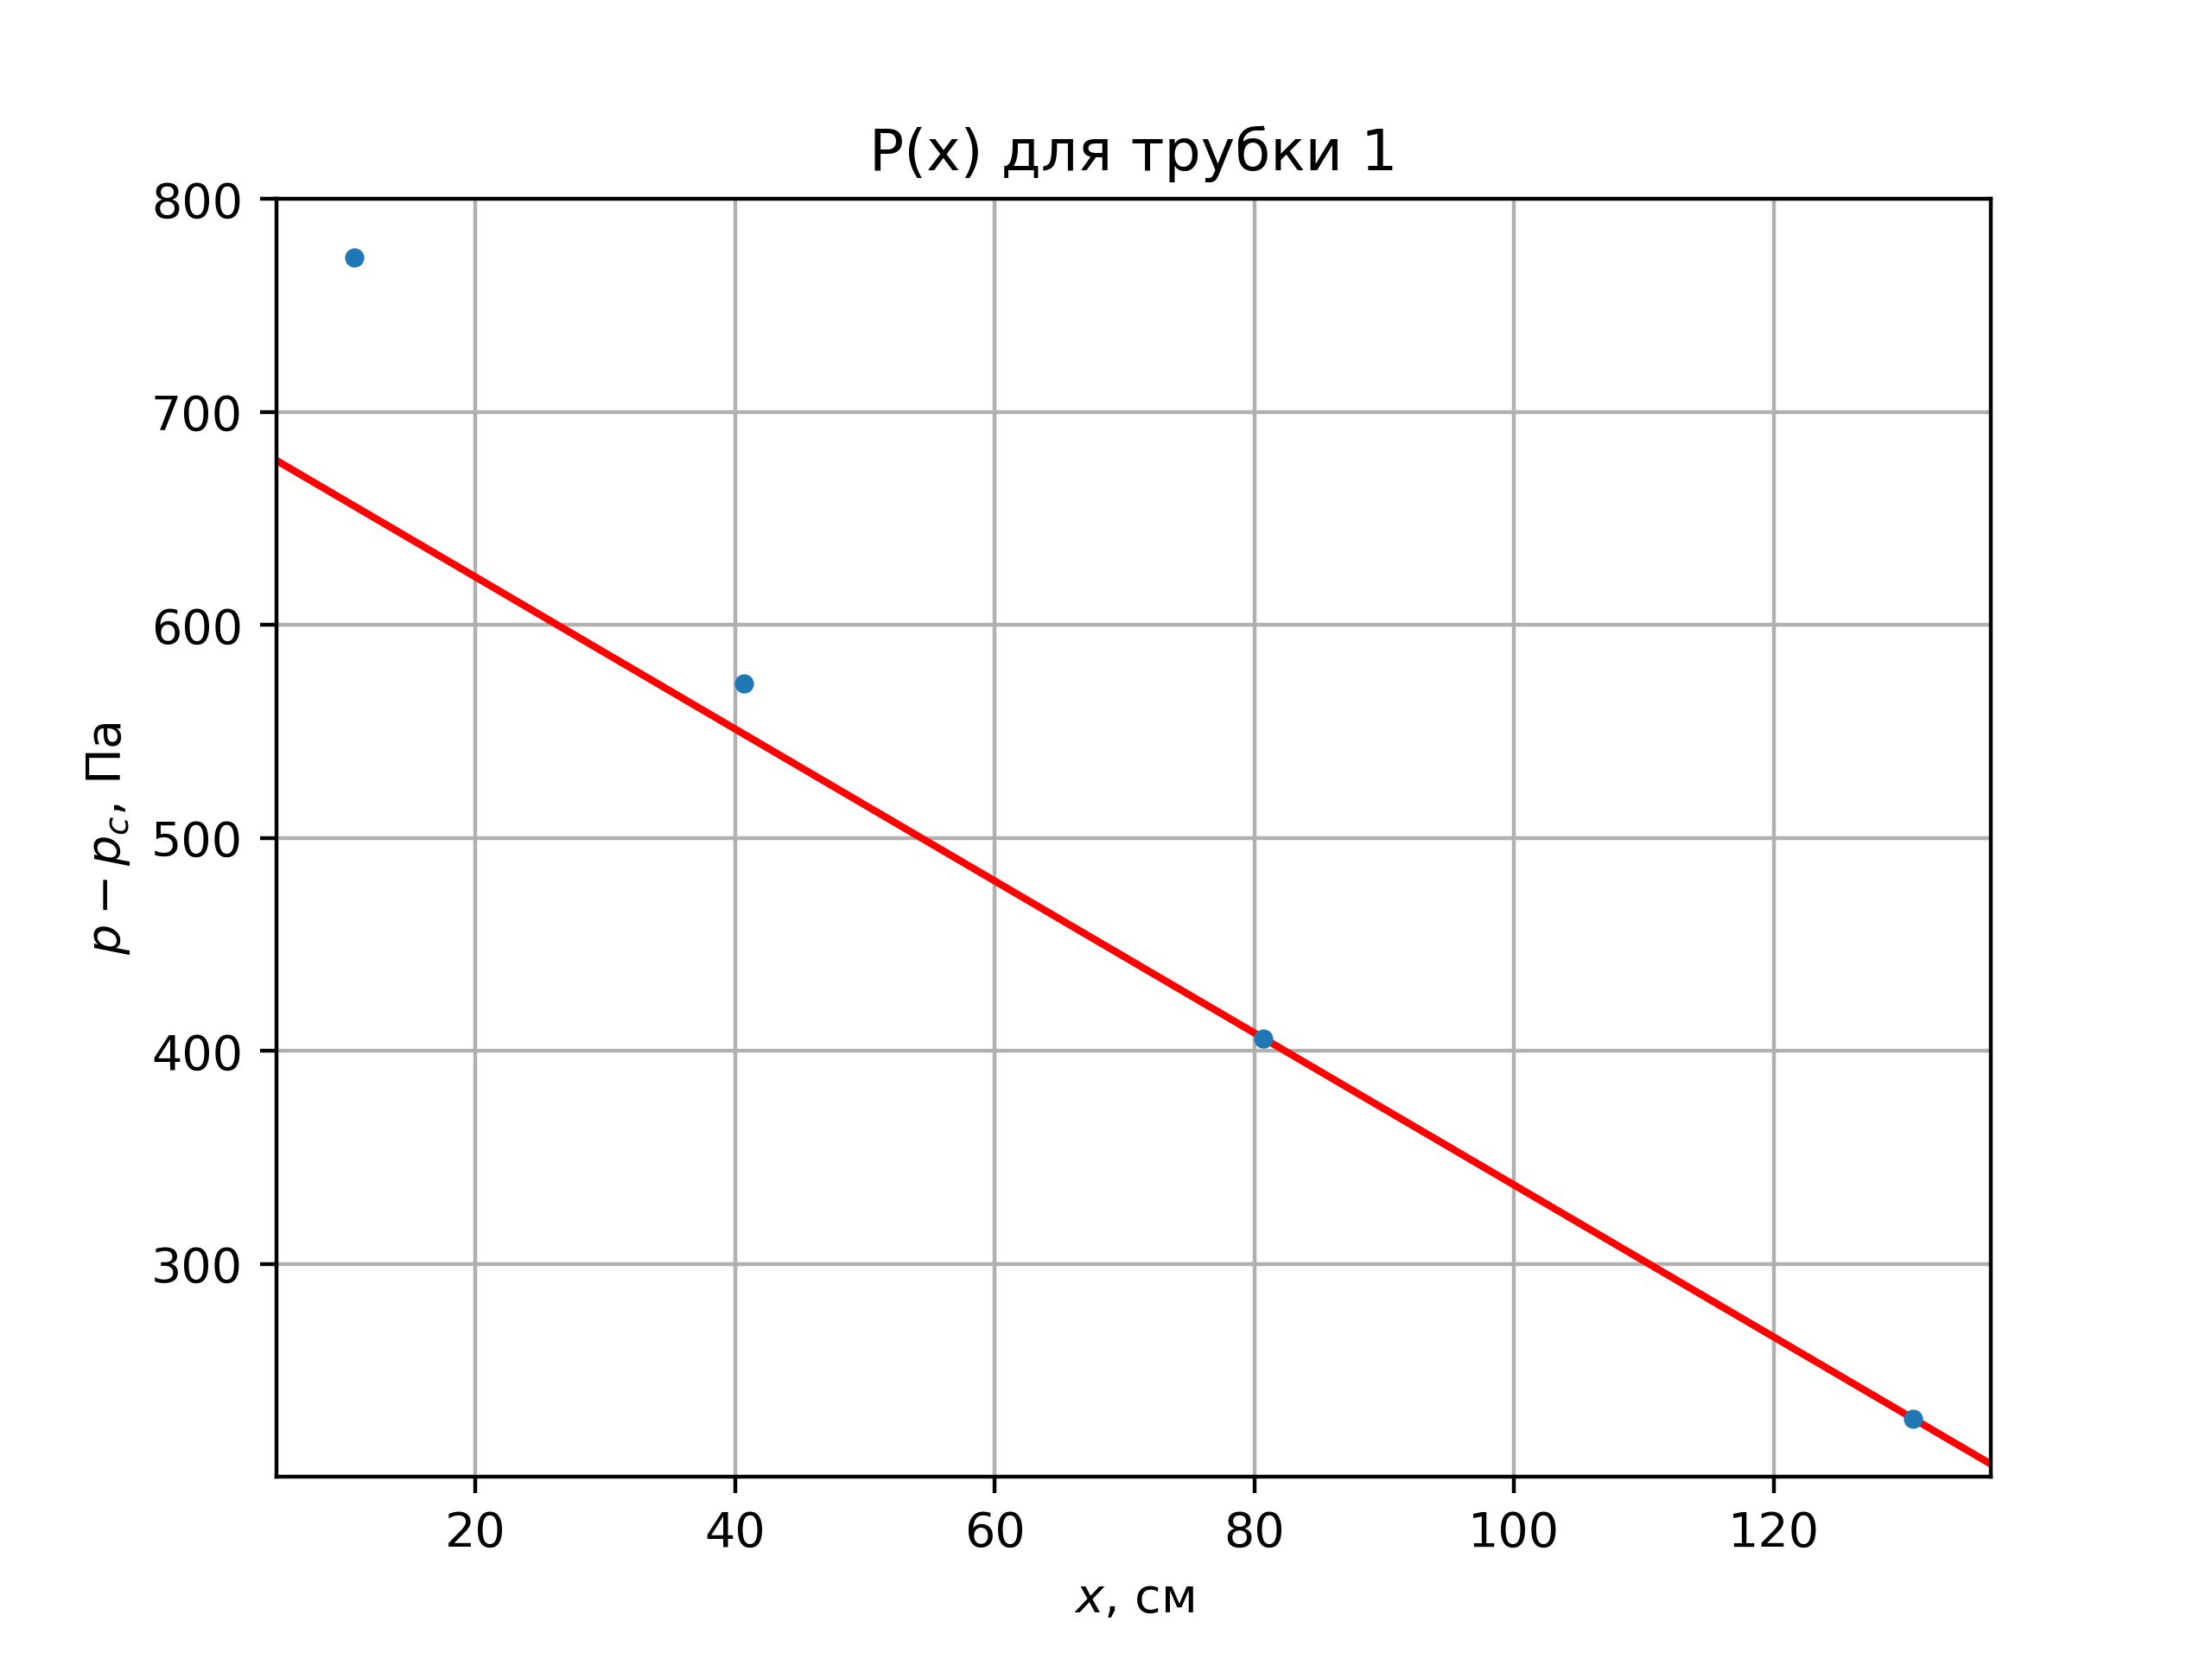
\includegraphics[width=0.5\linewidth]{img/data11.png}
    \centering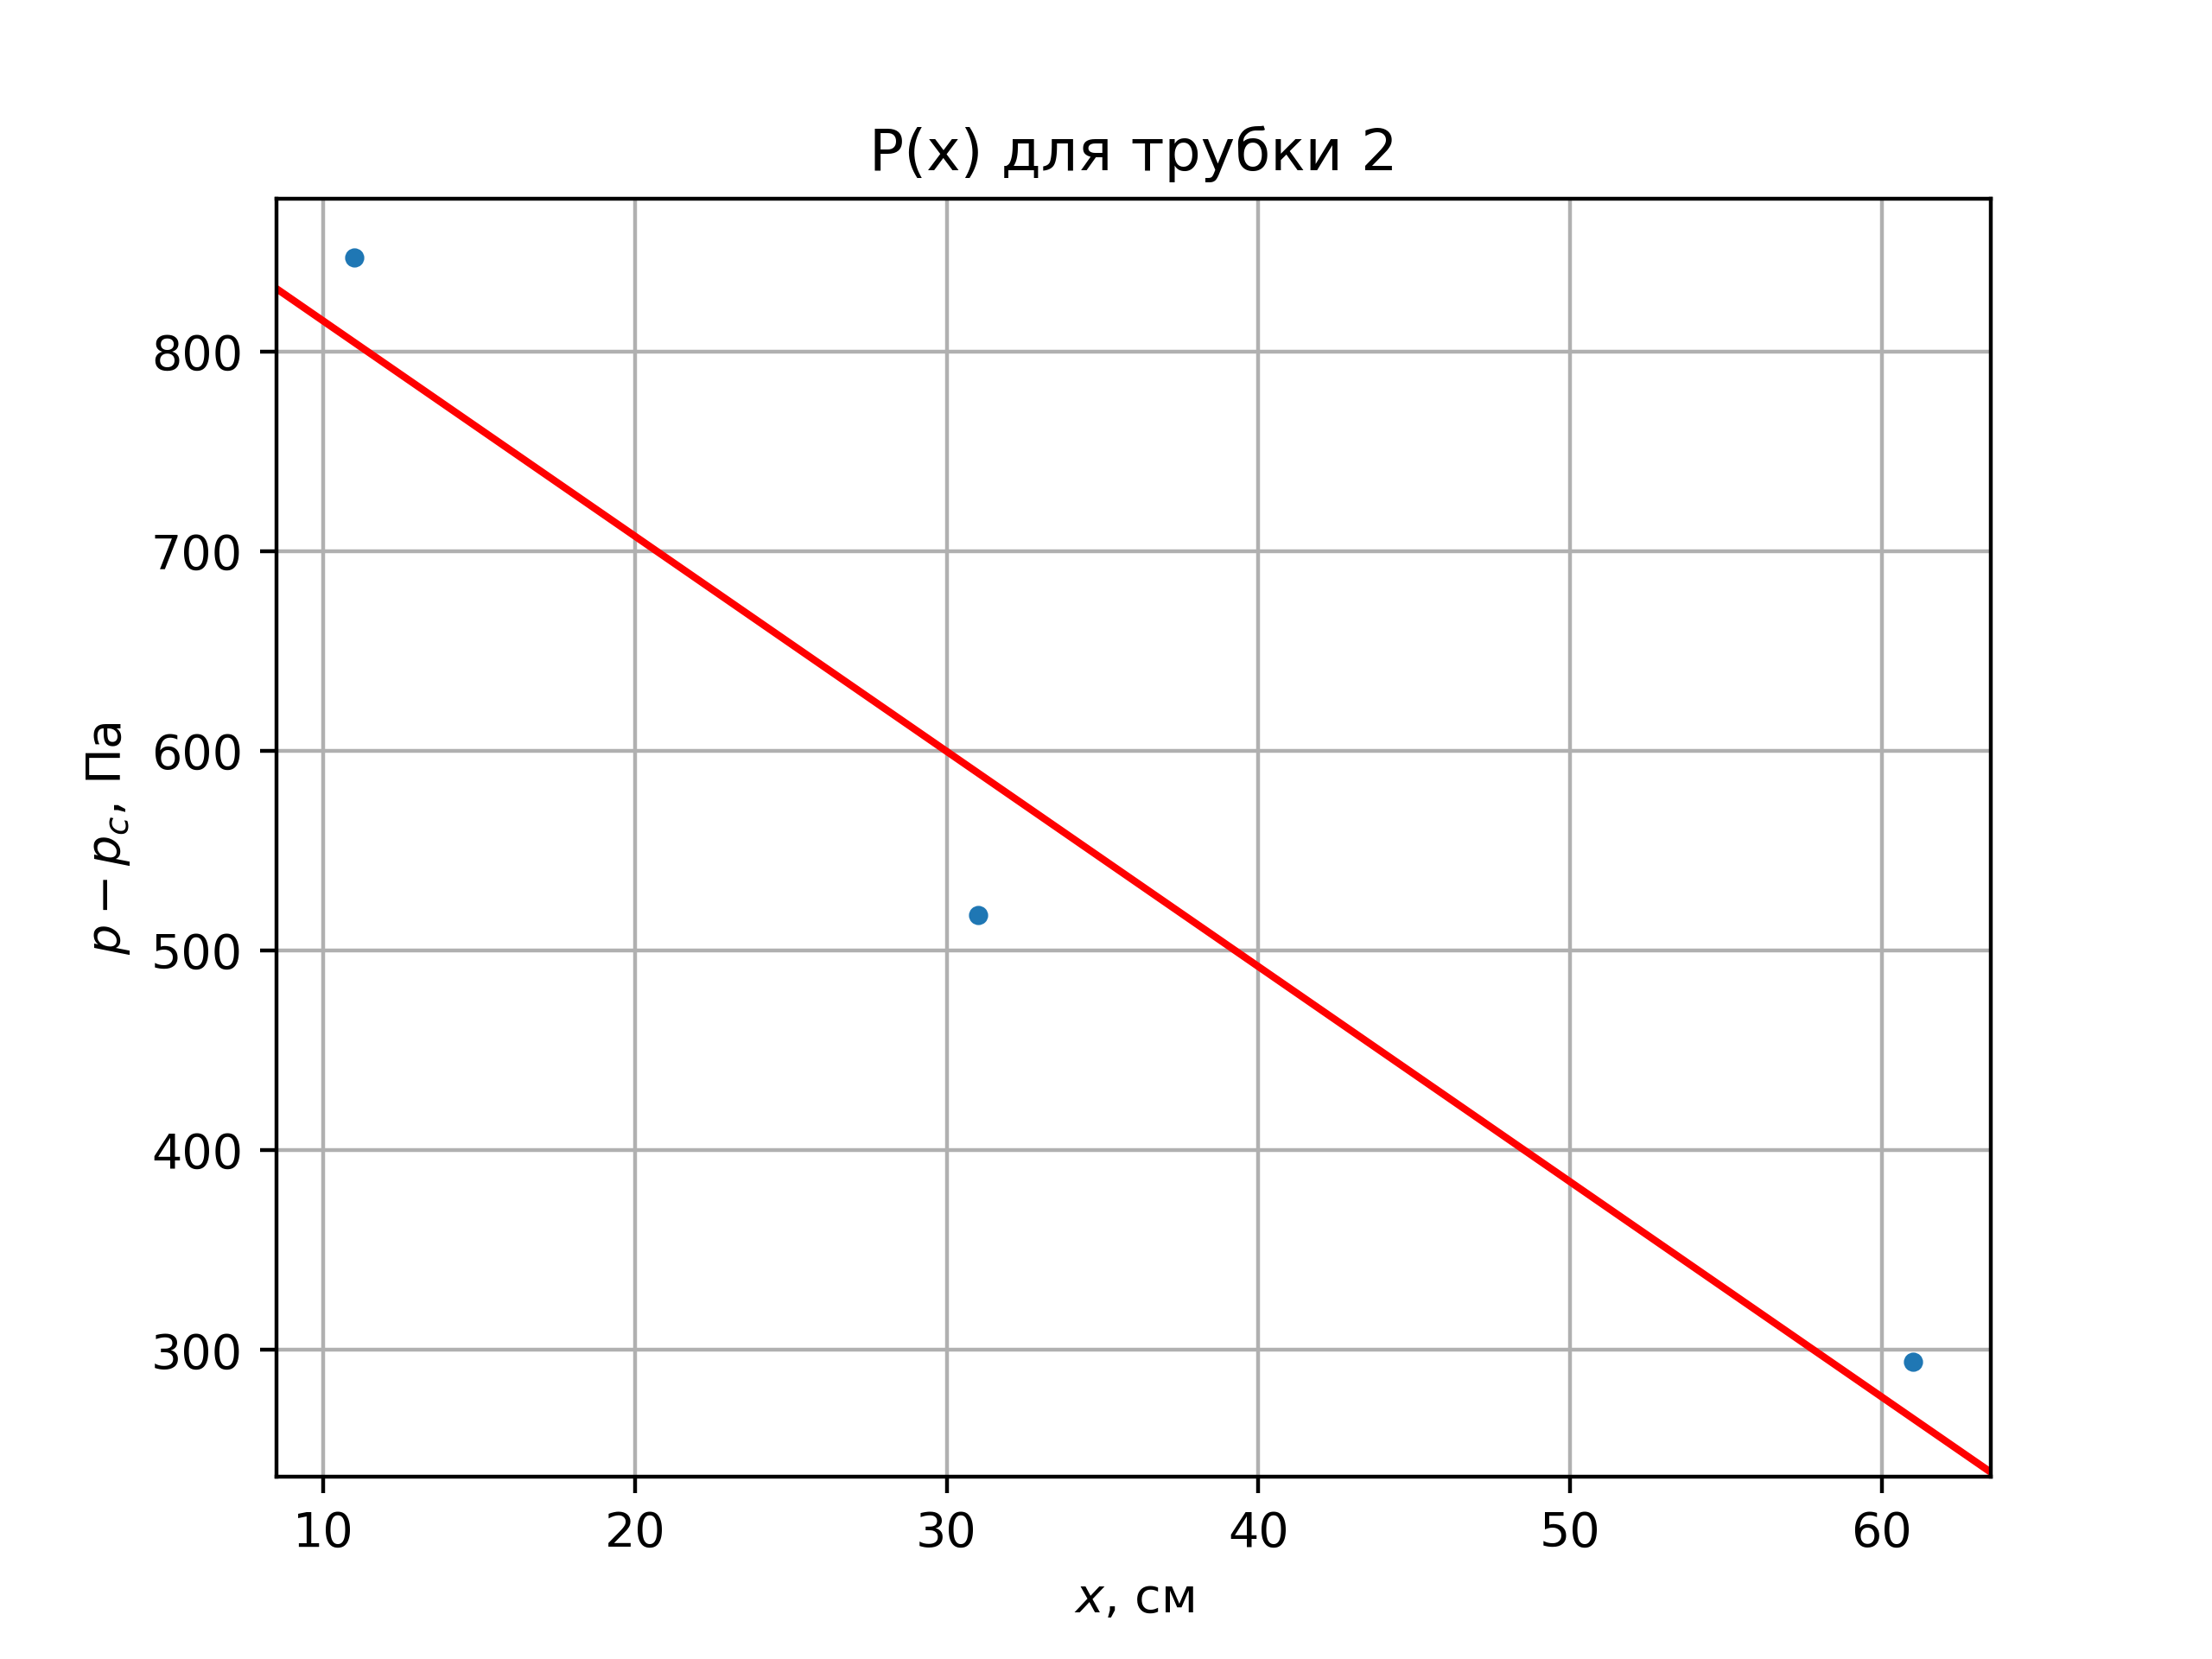
\includegraphics[width=0.5\linewidth]{img/data12.png}
    \centering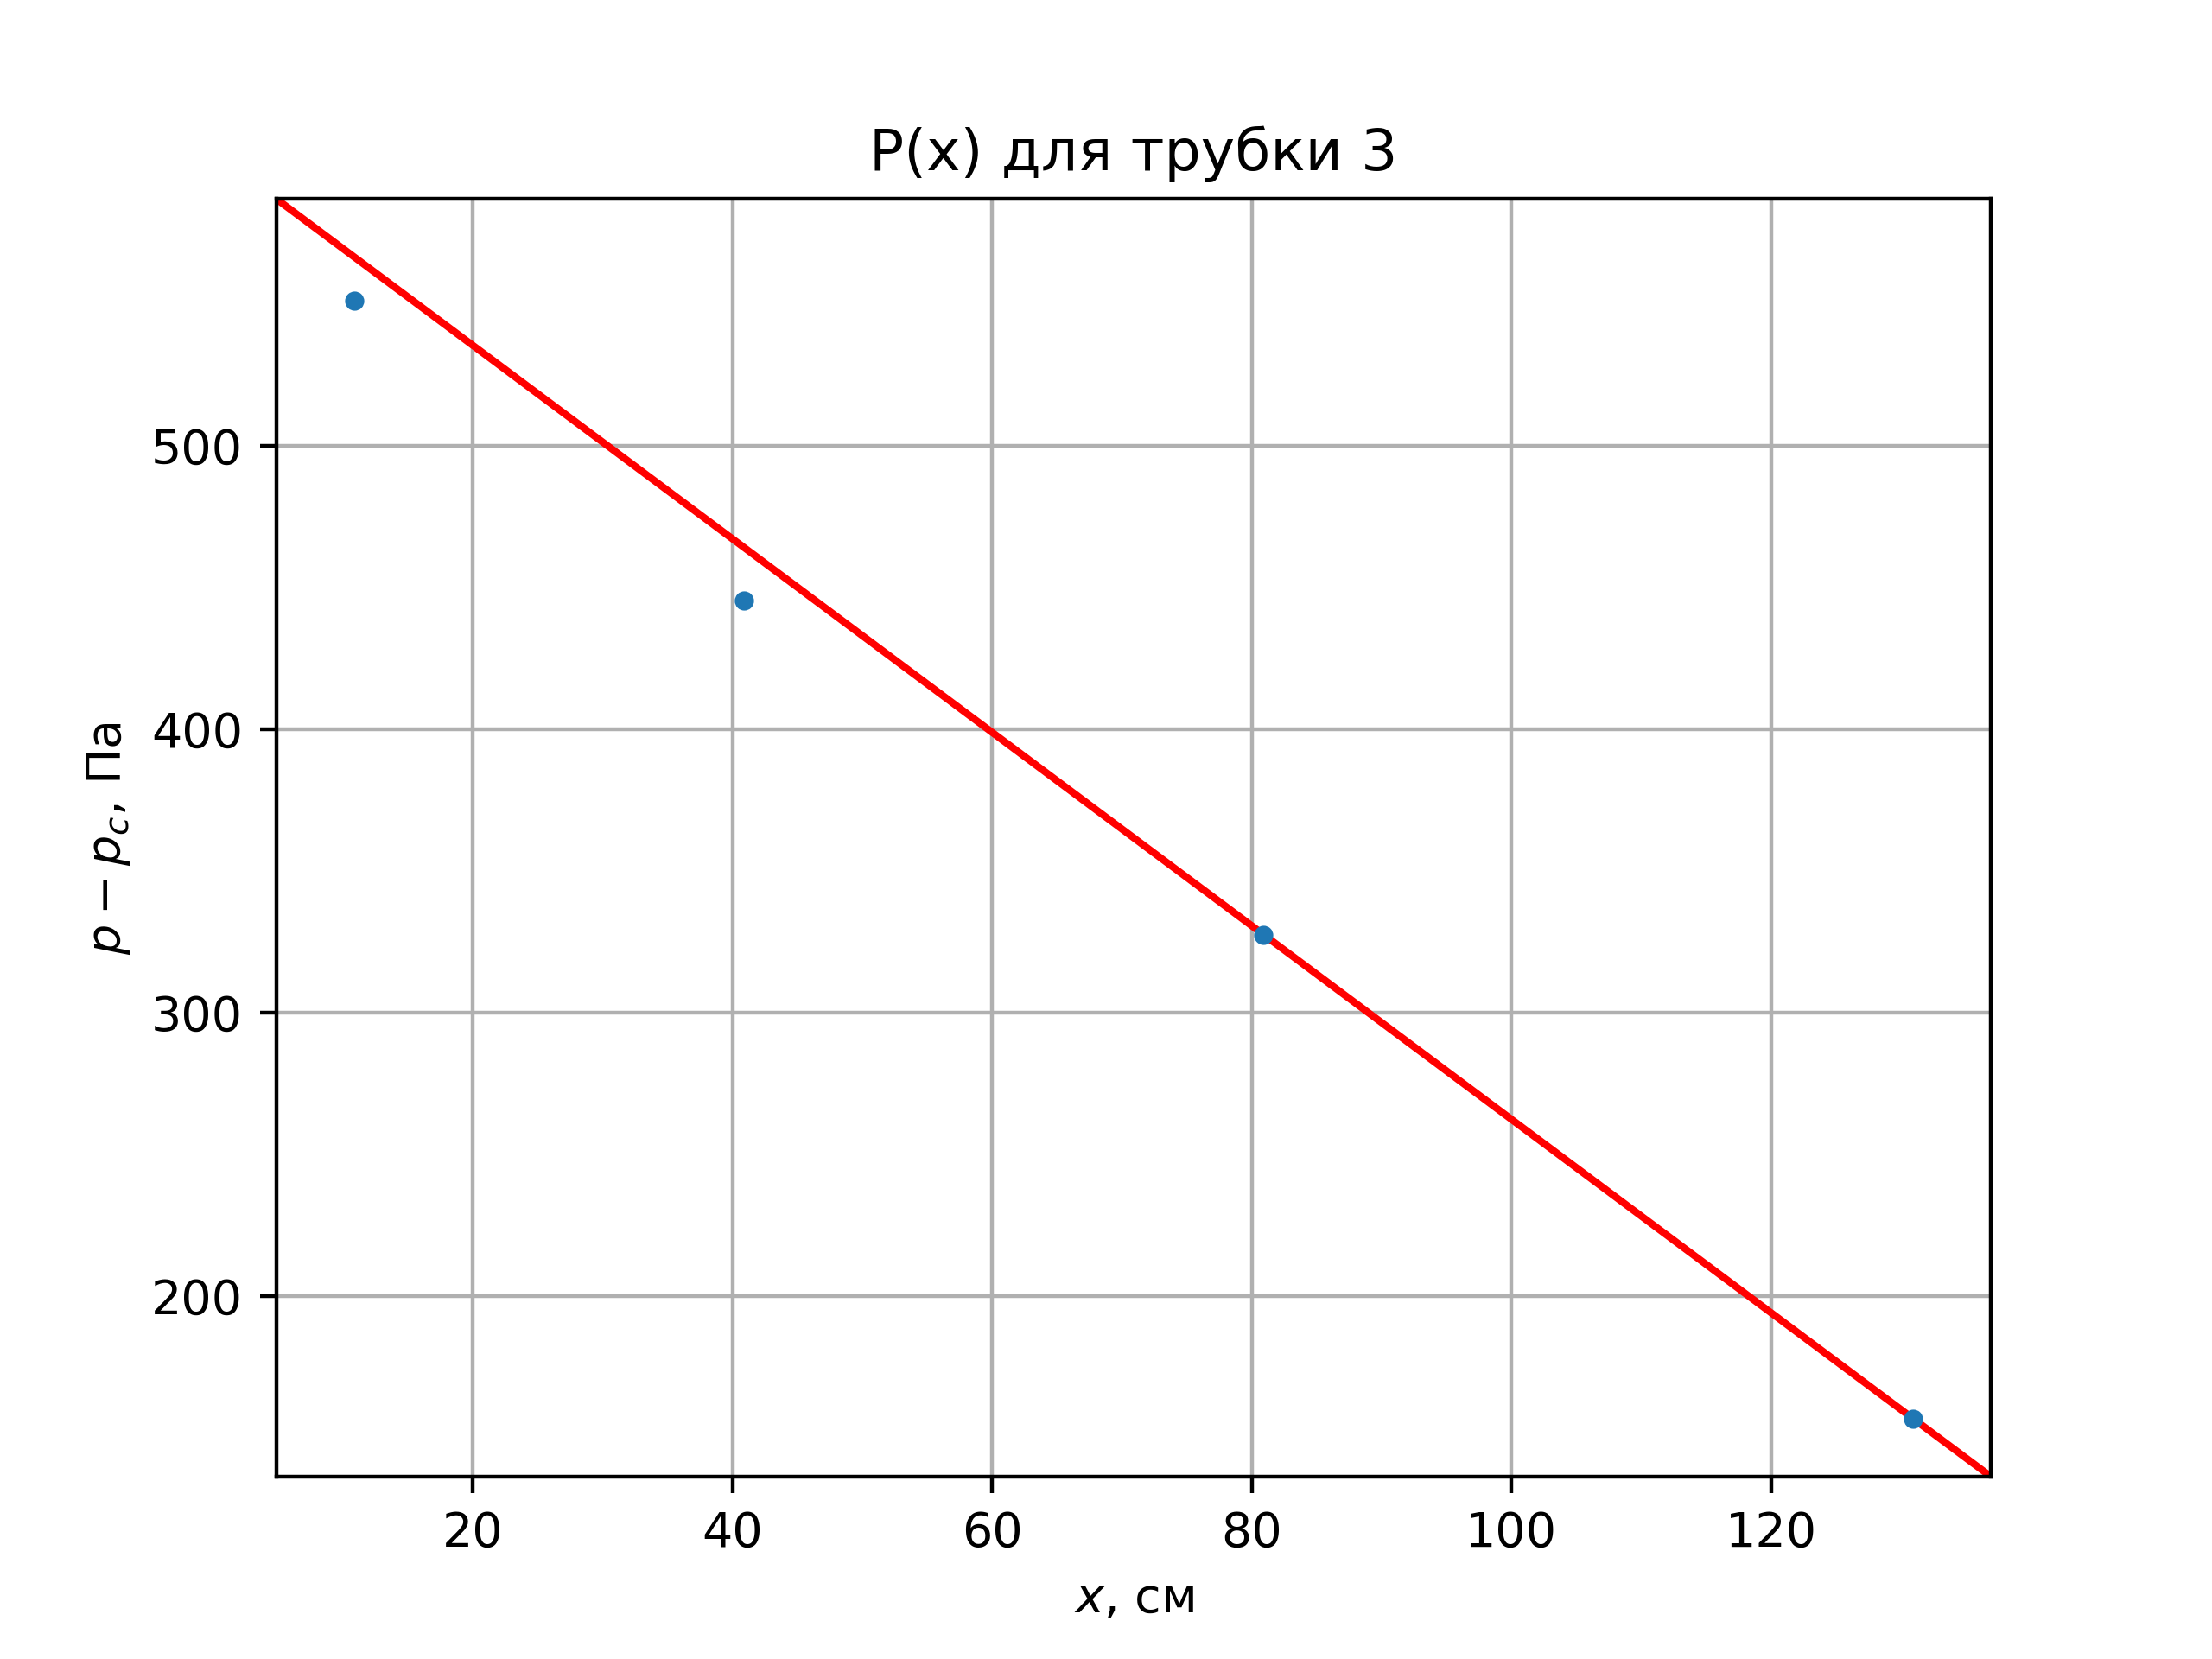
\includegraphics[width=0.5\linewidth]{img/data13.png}
\end{figure}

Как видно из графиков, сильное отклонение от линейной зависимости происходит
на расстояниях меньше 30--40 см, т.е. формула $l_\text{уст}\approx 0{,}2\cdot R\cdot\mathrm{Re}$
верна.

\begin{table}[!ht]
    \caption{Данные для ламинарного течения ($dp/dl\approx 98\,\text{Па}/\text{м}$)}
    \begin{tabular}{|l|l|l|l|}
    \hline
        $Q\,\text{л}.\text{с}$ & $l,\text{см}$ & $d\,\text{мм}$ & $\Delta d\,\text{мм}$ \\ \hline
        0.09683 & 50 & 5.25 & 0.05 \\ \hline
        0.02875 & 20 & 3 & 0.1 \\ \hline
        0.03186 & 50 & 3.9 & 0.05 \\ \hline
        0.10504 & 50 & 5.05 & 0.05 \\ \hline
        0.105 & 20 & 5.1 & 0.05 \\ \hline
        0.01108 & 15 & 3 & 0.1 \\ \hline
        0.0295 & 25 & 3.95 & 0.05 \\ \hline
    \end{tabular}
\end{table}

\begin{table}[!ht]
    \caption{Данные для турбулентного течения ($dp/dl\approx 490\,\text{Па}/\text{м}$)}
    \begin{tabular}{|l|l|l|l|}
    \hline
        $Q\,\text{л}.\text{с}$ & $l,\text{см}$ & $d\,\text{мм}$ & $\Delta d\,\text{мм}$ \\ \hline
        0.21975 & 50 & 5.25 & 0.005 \\ \hline
        0.09994 & 20 & 3 & 0.1 \\ \hline
        0.10633 & 50 & 3.9 & 0.05 \\ \hline
        0.22222 & 50 & 5.05 & 0.05 \\ \hline
        0.23126 & 125 & 5.1 & 0.05 \\ \hline
        0.06552 & 75 & 3 & 0.1 \\ \hline
        0.11366 & 125 & 3.95 & 0.05 \\ \hline
    \end{tabular}
\end{table}

\begin{figure}[ht!]
    \centering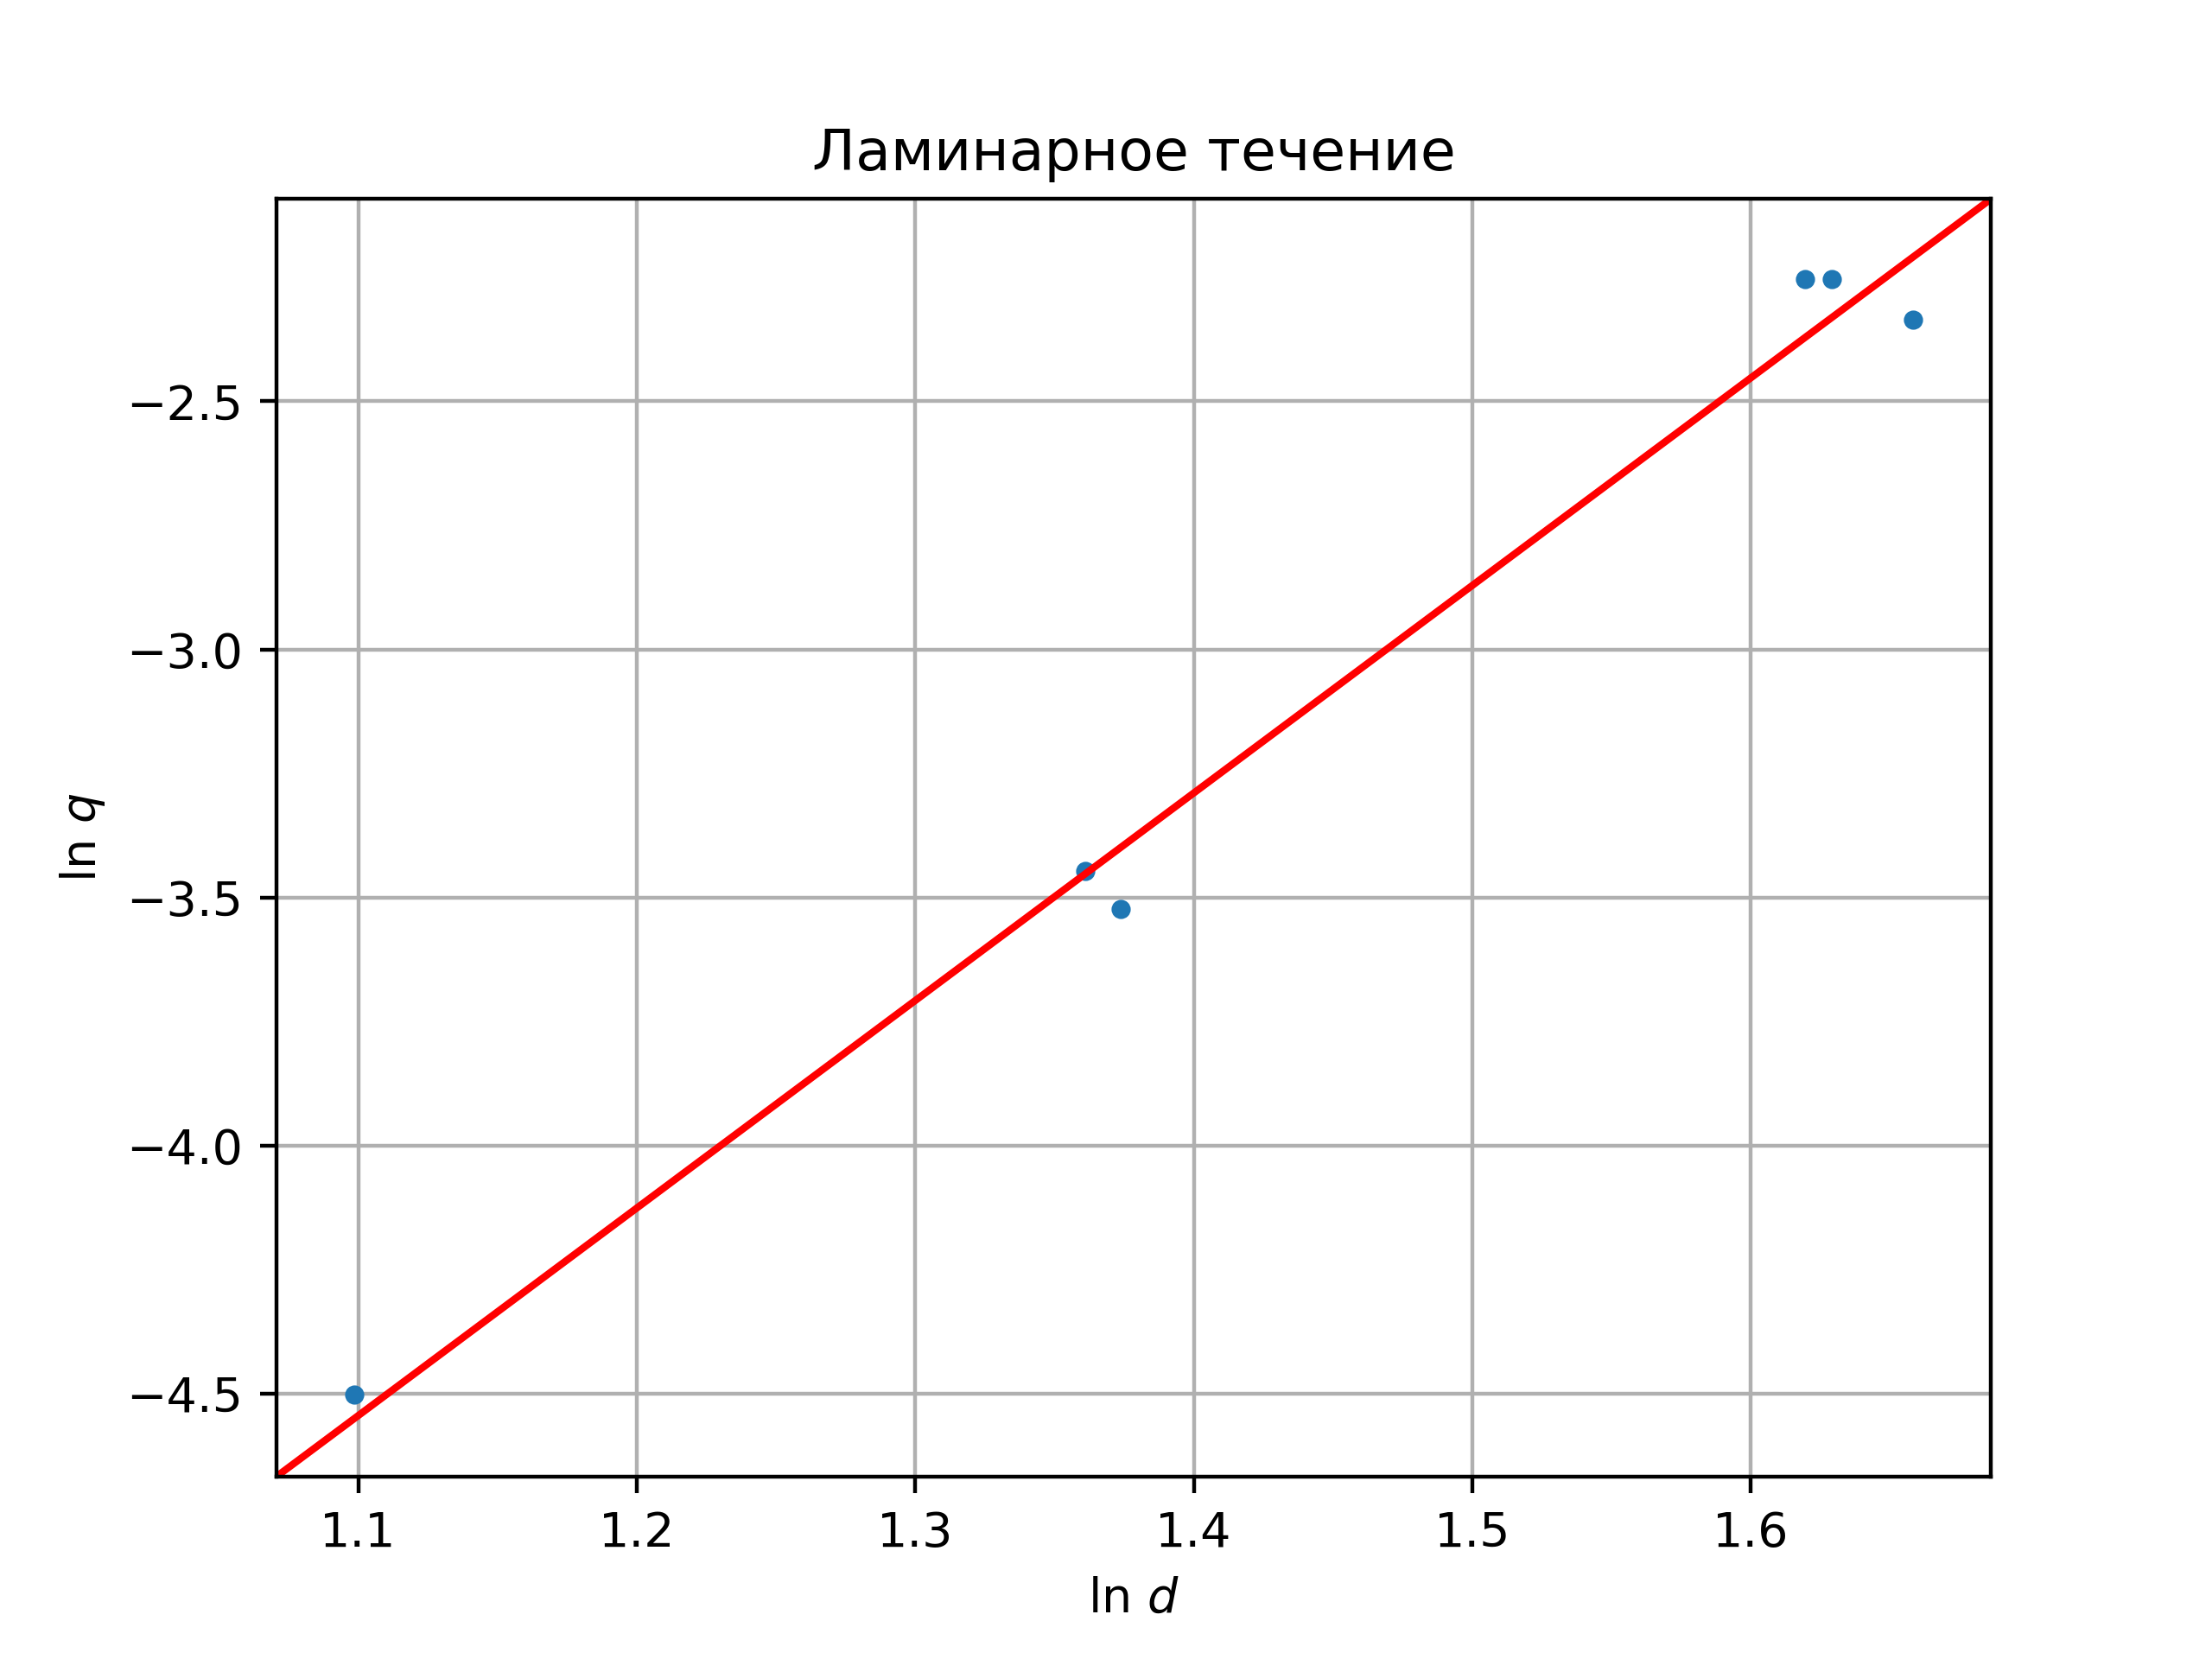
\includegraphics[width=0.8\linewidth]{img/lam.png}
    \centering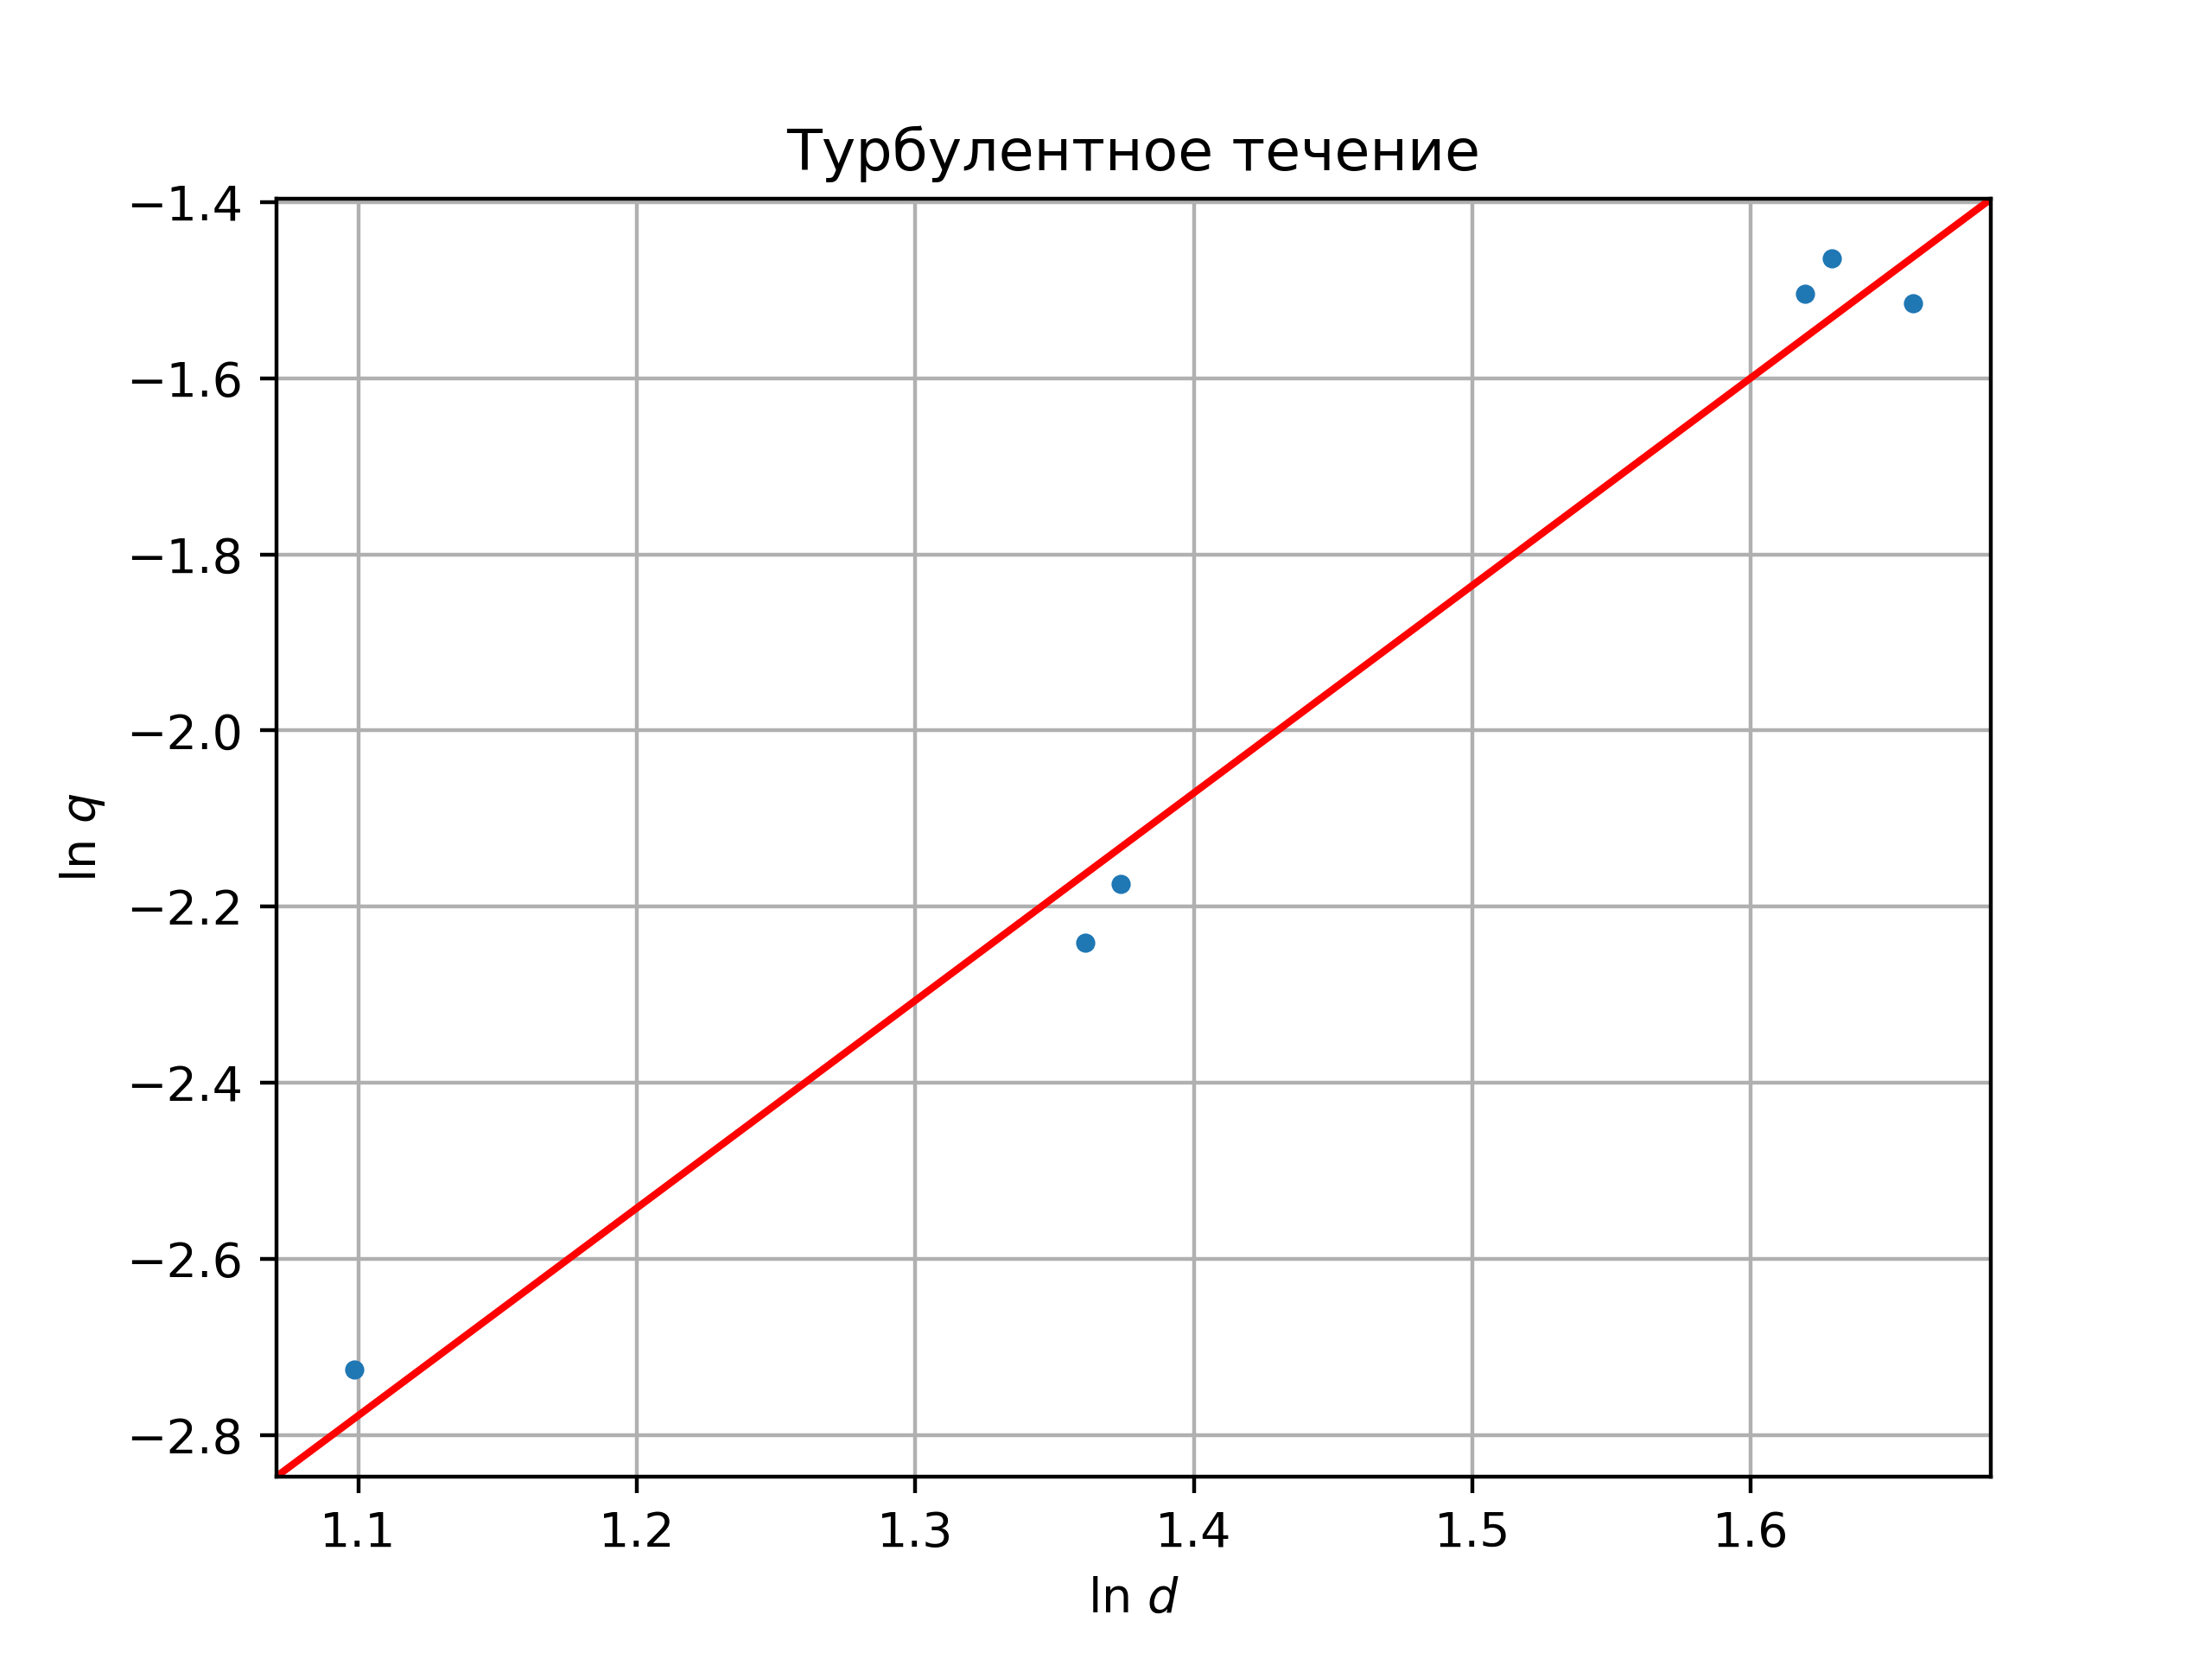
\includegraphics[width=0.8\linewidth]{img/tur.png}
\end{figure}

Наклон графика ламинарного течения $k=4{,}2\pm 0{,}2$, турбулентного $k=2{,}36\pm 0{,}15$,
что согласуется с теорией.
